\subsection{Problem Statement}

% A potential future use case, and 
A future use case of stochastic KV-SLAM would be for operations in environments which are intermittently occupied, e.g. factories, warehouses, office buildings, etc. The benefit of this method is that the robot can avoid operating during highly dynamic times, with the trade-off being that the environment may be significantly changed between sessions of operation. In the case of Astrobee, the navigation system was incapable of dealing with these inconsistencies between the internal map and the real world, regularly requiring astronaut assistance to recover. Trust in autonomous systems is already precarious, quickly falling upon the observation of failure \cite{robinetteEffectRobotPerformance2017}. Robotic SLAM failures can lead to navigational instability, task failure, and even the possibility of physical damage to the surrounding environment or the robot itself\cite{nahavandiComprehensiveReviewAutonomous2025a}. Therefore, in order for autonomous SLAM based robotic navigation to see widespread use, it must be accurate in its estimations, and capable of withstanding a wide variety of failure cases.

This research focuses on reducing failures caused by the existence of outdated map features in reused maps during stochastic KV-SLAM operations. For simplicity, we refer to the topic of reusing previously generated maps which have gone out of date as Outdated Map Reuse or OMR. There are three critical issues which appear in systems which do not handle the challenges of OMR sufficiently well. The first issue relates to the size of the map, as only adding newly observed features without removing outdated ones results in a monotonically increasing map size. This puts an ever-increasing strain on compute resources to deal with the large map, and increases the complexity of optimization steps. The second issue is in regard to relocalization, the process by which a KV-SLAM system redetermines its position within the map after being lost. The process of relocalization starts by identifying candidate positions within the map which are visually similar to the current camera image. A high proportion of outdated map points in the map interferes with this candidate selection, as the map's understanding of the visual features of the environment no longer match reality. The final issue affects the RANSAC process, a function which is run regularly as part of the process of determining the 3D transformation between successive frames. The RANSAC algorithm selects a random sample of points from the map and the new image to be localized, and attempts to determine a consistent 3D transformation which explains the correspondence. High proportions of outdated map points increase the risks of the RANSAC algorithm failing to find a consistent pose for the new frame, even if one exists. The map representation, relocalization, and RANSAC will be covered in greater detail in Section \ref{sec:kv_slam_background}.

There are two ways to prevent the failures attributable to OMR in KV-SLAM, both relating to the removal of map points. The first option is to proactively prevent map features which have potential to become outdated (i.e. they are located on an object that can move) from ever entering the map (i.e. the map will never be outdated because no features in the map can move). The second option is to retroactively identify and remove outdated features from the map once it has been loaded for reuse. The mechanism at play in the proactive case tends to be semantic identification and segmentation of input images, allowing semantic labels to determine whether map points which fall on certain objects are kept or not. These semantic processes require significant compute and storage resources, often making them unsuitable for compute constrained applications such as small scale mobile autonomous vehicles (MAVs). In the reactive case, the methods stray away from the field of semantics, and towards the field of change detection. These methods work by identifying inconsistencies between the map and the camera observations, flagging points for removal once confidence in their existence drops below some threshold. However, a gap can be noticed in the change detection methods available today. This operation of removing map points based on some criteria comes up a lot in SLAM, and will be referred to Map Point Removal or MPR throughout this research. While change detection methods do collect point-level metadata, to the researcher's knowledge, no change detection methods collect metadata on the global observability of each map point, leaving today's systems susceptible to overzealously flagging map points which are temporarily obstructed from certain viewpoints for removal. The semantic and change-detection methods will be discussed in greater detail in Section \ref{sec:related_work}.

\begin{figure}[h!]
    \centering
    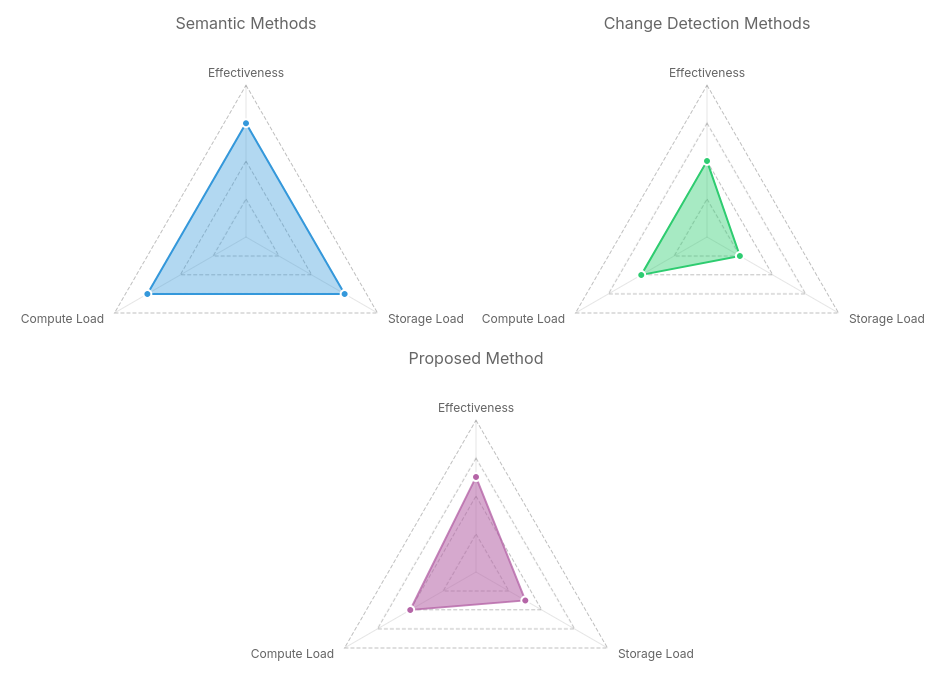
\includegraphics[width=0.8\textwidth]{resources/omr_method_comparison.png}
    \caption[OMR Method Comparison]{A qualitative comparison of compute load, storage load, and effectiveness between various OMR point removal methods.}
    \label{fig:omr_method_comparison}
\end{figure}

The key takeaway is that OMR can greatly benefit stochastic KV-SLAM systems, but without properly handling the outdated data, OMR systems create new failure cases which degrade the system's performance. The methods available which allow OMR to be successfully integrated make a trade-off between computational requirements, storage requirements, and effectiveness as illustrated in Figure \ref{fig:omr_method_comparison}. As an engineering problem, the constraints which will drive the decision of methodology for MPR are size, weight, power, and cost. It is not always possible to just u It is the conjecture of this research that a novel change detection method which stores the global observability of map features at the point level could improve upon the effectiveness of existing change detection techniques, without a significant increase in computational load or storage requirements.